%!TEX root = ../template.tex
%%%%%%%%%%%%%%%%%%%%%%%%%%%%%%%%%%%%%%%%%%%%%%%%%%%%%%%%%%%%%%%%%%%%
%% chapter4.tex
%% NOVA thesis document file
%%
%% Chapter with lots of dummy text
%%%%%%%%%%%%%%%%%%%%%%%%%%%%%%%%%%%%%%%%%%%%%%%%%%%%%%%%%%%%%%%%%%%%

\typeout{NT FILE chapter4.tex}%

\chapter{Related Work}
\label{cha:related_work}

\section{Web API Description Languages} % (fold)
\label{sec:web_api_description_languages}

Web service development has risen dramatically in recent years,  unlike statically linked library APIs,
where developers may choose to stick with an earlier version that met their needs, with web APIs,
the provider can discontinue a specific version and capability at any moment, changes are immediate and irreversible.
This represents a heavy burden for developers of client modules as it causes an endless struggle to keep up
with changes pushed by the web API providers.
This load is exacerbated if the web API is inadequately documented.

Web API Description Languages (WADL)~\cite{webapi} are domain-specific languages used to describe web service contracts in a standardized structure;
also sometimes more generally referred to as interface description languages (IDLs).
These structured descriptions may be used to produce documentation for human programmers, that is easier to read than free-form documentation,
because all the generated documentation adheres the formatting norms set by the used tool.
Furthermore, description languages are often accurate enough to allow for the automatic generation of various software artifacts such as mock servers,
client code generation in different programming languages, load test scripts, and so on.

The OpenAPI Specification (OAS)~\cite{openAPI} is the most widely adopted Http Description Language;
it defines a standard language-agnostic interface that allows both computers and humans to comprehend the capabilities of a service.
The OpenAPI initiative is on a continuous effort to develop API tooling on top of their specification, some of the supported tools of version 3.0 range from:
\begin{itemize}
    \setlength\itemsep{0em}
    \item Auto Generators: Tools that parse code and turn it into an OpenAPI Specification document
    \item Mock Servers: Fake servers that take the description document as input, then route incoming HTTP requests to example responses or dynamically generates examples.
    \item Data Validators: Verify if API requests and responses are lining up with the API description.
    \item Security: Tools that can look out for attack vectors by inspecting OpenAPI descriptions.
    \item Converters: Various tools to convert to and from OpenAPI and other API description formats.
\end{itemize}

OpenApi allows a detailed description of the syntactic aspects of the data transferred, however it ignores semantic aspects, such as the ability to relate
different parts of the same data, to relate the input against the state of the service, and the output against the input.
For instance, OpenAPI does not allow developers to indicate that in the creation of a new user, the nickname must be shorter
than the full name.

\citeauthor{headRest}~\cite{headRest} proposes an alternative WADL that supports the expression of semantic aspects in data, the HeadRest specification language.
Two ideas are embodied in the proposed language:

\paragraph{Refinement Types~\cite{freeman1991refinement}} can be used to express the properties of data exchanged.
A refinement type x can be defined as
\[ x:T \rightarrow e \]
Where x is an object of the primitive type T, and e is a predicate which returns true or false depending on whether the value conforms to the boolean expression (e.g.\ x > 10).

\paragraph{Pre- and post-conditions}can be used to express relationships between data sent in
requests, and the data returned in responses. These conditions can be expressed as a collection of Hoare triple assertions
\[ \{\phi\} (a : t) \{\psi\} \]
Where \emph{a} is HTTP operation type (GET, POST, PUT, or DELETE), \emph{t} is an URI template (e.g. /users/), and $\Phi$ and $\Psi$ are boolean expressions.
Formula $\Phi$, called the pre-condition, addresses the state in which the action is performed as well as the data transmitted in the request,
whereas $\Psi$, the post-condition, addresses the state resulting from the execution of the operation together with the values transmitted in the response.

Web API description languages provide a foundation for defining compatibility relations between service contracts in the evolution description language,
presented further ahead in Section \ref{sec:evolution_specification}.

\section{Schema Representation Languages} % (fold)
\label{sec:schema_representation_languages}

Schema representation languages (SL)~\cite{schemalanguagetaxonomy} are used to specify and document the structure and semantics of data.
A schema language is typically backed by a serialization protocol, which is used when data must be transported across a network or stored with durability.
Some serialization protocols do not have a well-defined schema language.
This is the case in the serialization libraries provided by programming languages, which serialize data in a native binary format that is not human-readable.
In the setting of microservices, serialization libraries supplied by programming languages are strongly discouraged,
because each service may be written in a different programming language.
Data consumers will be unable to comprehend producers if they use mismatching data representations.

Cross-language serialization libraries, such as JSON~\cite{json}, can solve this problem.
However, cross-language formats typically don't have the same level of expressiveness as the programming languages that employ's them,
making data consumption more difficult due to poor type-safety guarantees.
For example, whereas Java offers distinct data types that differentiate integers from floating point values, JSON regards them as the same data type.
In the above case, if no further documentation is supplied, consumers will be constrained to adopt the more embracing data type "float" in order to avoid runtime errors.

JSON also doesn't have a well-defined schema language.
In JSON schemas are typically inferred from the structure of objects in a programming language that represent the received and sent messages.
Without an explicit schema definition and versioning strategy, fields can be unilaterally added or withdrawn at any moment without the consumers' knowledge.

There are cross-language serialization protocols that require the data schemas to be explicitly defined under schema language.
Avro~\cite{8}, Thrift~\cite{9}, and Protocol Buffers~\cite{10} are among them.
The benefit of having an explicit and versioned schema is that it makes the system more robust to schema evolutions, and
enables messages to be sent with minimal size.
The encoding of a message only requires the inclusion of the message data, and the schema version.
A service can be made aware of a message complete schema prior to receiving it via a schema registry.
The inclusion of information about each field's data type and name is redundant,
and it is only useful if the message is meant to be human-readable in an environment where the message schema is inaccessible.

Schema representation languages are a part of the specification of service contracts
presented further ahead in Section~\ref{sec:contract_specification}.

\section{Schema Registry} % (fold)
\label{sec:schema_registry}

A schema registry, as the name implies, is a repository for schemas.
It stores a versioned history of schemas and provides an interface for retrieving, registering, as well as checking the compliance of schemas.
It is essentially a CRUD (Create, Read, Update, Delete) application with persistent storage for schema definitions, where each schema is given a unique ID.

One framework that employs schema registries is Avro~\cite{8}, a data serialization framework developed within Apache's Hadoop project.
Avro requires a schema registry because the encoding of data records does not include data about the record structure such as field names or data types.
Only the data values of a record are appended in the serialized byte sequence, as seen in Figure~\ref{fig:avro}.
The deserializer knows which bytes belong to which field by comparing both the consumer and producer schemas.
This allows for a more compact serialization method, but it requires data consumers to understand the structure of the data written by producers.

\begin{figure}[htbp]
    \centering
    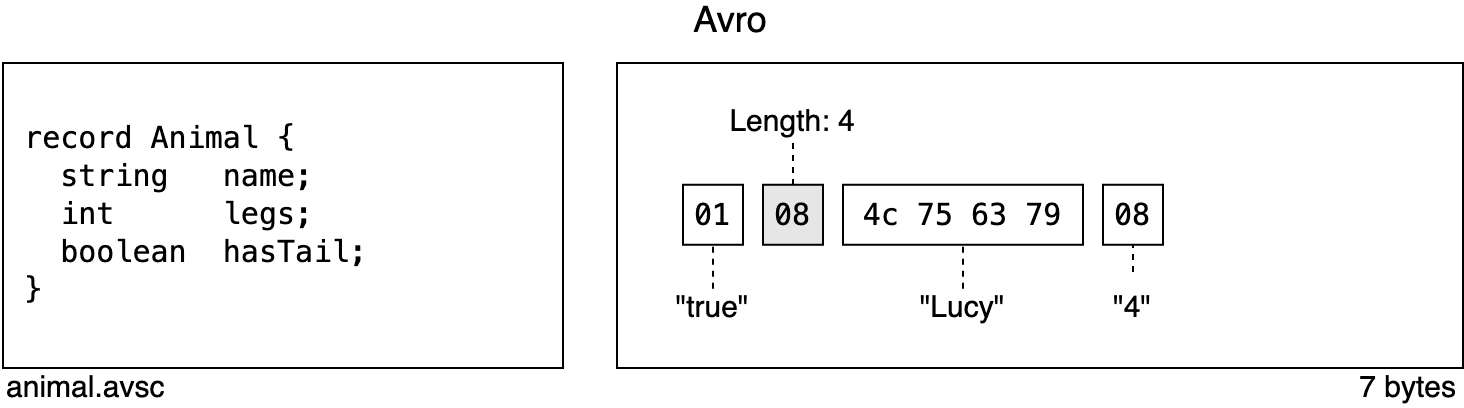
\includegraphics[height=1.5in]{avro}
    \caption{A Avro schema and its associated serialized record }
    \label{fig:avro}
\end{figure}

Another system that makes use of schema registries, is the Java RMI \cite{12},
a Java API that supports remote procedure calls (RPC) with distributed garbage-collection.
The Java RMI makes use of a schema registry to enable clients to obtain a references (stubs) to a remote objects.
In the RMI the registry is only used for locating the first object that a client needs, each reply from the registry provides
support for finding other objects.

Registries can be used to store not only service schemas but also service-to-service dependencies, and other meta-information about services, the benefits and drawbacks of their use will be
assessed in Section \ref{sec:tools}.

\section{Service Evolution Approaches} % (fold)
\label{sec:service_evolution_approaches}

Controlling and supporting the evolution of services is a significant technological research endeavor.
\citeauthor{webServiceEvolution} \cite{webServiceEvolution} propose five standards for evaluating existing methods for evolving Web services.
These standards and some methods are also applicable in a microservice setting:
\begin{itemize}
    \item \textbf{Granularity of evolution -} Granularity refers to the unit on which the evolution is based.
    Coarse-grained evolution strategies support the evolution of general interface properties,
    whereas fine-grained evolution strategies support the evolution individual basic properties, such as the type of parameter in a method.
    \item \textbf{Terminal of evolution -} The term refers to whether the end result of a changed service affects the producer, the consumer, or both.
    \item \textbf{Type of evolution -} Evolutionary methods can be divided into two broad categories: semantic and architectural.
    Architectural methods typically support changes in the composition of components, whereas semantic methods are primarily based on the semantic extension of contracts.
    \item \textbf{Scalability -} This standard assesses an evolutionary method's applicability and generality in different contexts.
    \item \textbf{Maintainability -} This standard assesses the difficulty of maintaining system's that employ the relevant evolutionary method.
\end{itemize}

Below, it is presented a summary of the common approaches used to support the evolution of microservices,
along with their strengths and shortcomings in regard to the standards outlined above.

\subsection{Hand-off Period} % (fold)
\label{sec:hand_off_period}

The conventional approach for evolving microservices is to keep deployments of service versions that are still being consumed available with a hand-off period,
and to route requests to the service deployment that has the appropriate version.
This approach has been proven to be pragmatic, but exceedingly expensive,
because it necessitates high maintainability and partitions available resources among continually shifting subsets of consumers.

\subsection{Deprecated Endpoints} % (fold)
\label{sec:deprecated_endpoints}

Alternatively it's possible to support backwards compatibility without distinct deployments,
by including in the new service contract the endpoints of the prior service versions that are still in use.
When a breaking change occurs in a contract evolution, we preserve the old endpoint and implement the new endpoint separately.
The old endpoint is not modified and is still accessible via a similar but distinct path.

Contract changes that only affect HTTP parameters can easily be accommodated under this approach, however, contract changes that affect
request body schemas are problematic because it would be necessary to write distinct serialization and de-serialization rules for each version of the schema.
This approach can add significant amount of effort to the development team because each breaking change requires all the serialization rules to be rebuilt,
in order to support the format of the new revised schemas.
Schemas with multiple serialization rules also tend to become unreadable.
Furthermore, this approach doesn't offer any safety guarantees,
a developer might easily make the error of deleting a serialization rule that is still in use.

\subsection{Schema Resolution Rules} % (fold)
\label{sec:schema_resolution_rules}

The previous approach can be complemented with the use of sophisticated serialization protocols such as Avro, Protocol Buffers or Thrift.
These protocols support the evolution of schemas via resolution rules and declarative semantics,
where the old version of the software can deal with the new version of the service’s syntax.
However, the schema evolution support in these protocols is limited \cite{11}.
The common limitations of the aforementioned protocols are presented bellow:
\begin{itemize}
    \item To ensure backwards compatibility, newly added fields must be optional.
    \item The only fields that can be removed to maintain forward compatibility are optional fields.
    \item It's not possible to change a field type or its format freely, field types can only be promoted to more embracing types (e.g int\textrightarrow float).
    \item Renaming fields is supported through the use of aliases that cannot be re-used by other fields in the same scope.
\end{itemize}

In the context of microservices, backward compatibility is only required in request schemas, while forward compatibility is only required in response schemas.
In other words the current producer implementation must be able to interpret request messages from outdated consumers, and outdated consumers
must be able to interpret response messages from the current producer implementation.
Schemas that are used both in request and response messages most support forward and backward compatibility.

Optional fields are imposed in the above cases due to missing information in messages.
If a field must be required, its value can be supplied through static default values.
All fields that are optional exclusively because of limitations in resolution rules should be treated as required when a consumer and producer agree on the same schema version.
Since there is no absence of information, the default value should not be used in this case.
To simply put it, the system should enforce required fields when the consumer and producer agree on the same schema, and only use static default values when the consumer and producer disagree.

The aforementioned protocols do not differentiate between the two cases; instead, their resolution rules solely operate over the syntax of schemas and are agnostic to the version of the consumer and producer's schema.
In order to enforce required fields in the former case,
validation logic would need to be written repeatedly by programmers (in the same layer as the business logic).
This validation should be in a layer above because, the scale of the validation logic is proportional to the complexity of messages being validated;
for messages with more properties, particularly those with nested objects, the validation footprint can rise dramatically in terms of both line-count and logical complexity.

There are serialization protocols with built-in support for the evolution of contracts based on Event-driven and RPC communication methods.
However, if the HTTP communication protocol is adopted, serialization protocols will be unable to manage changes in the signature of endpoints (e.g. changing the method of HTTP endpoint's from GET to POST),
only changes in schemas of a message body will be managed in this case.
To support the evolution of endpoint signatures, this approach will need to be supplemented the deprecation of endpoints discussed above.
To decrease the complexity of contract evolutions, it is beneficial to handle both the evolution of schemas, and the evolution of endpoint signatures in a single integrated approach.

\subsection{Chain of adapters} % (fold)
\label{sec:chain_of_adapters}

The chain of adapters is a design strategy for supporting web services in the face of independently developed and unsupervised external consumers while preserving strict backwards compatibility.
This approach decomposes long update/rollback transactions into smaller, independent transactions.
This technique is discussed in depth by \citeauthor{13} \cite{13}.
The key concepts of the approach are presented bellow.

The service's backwards compatibility is ensured by the composition of adapters in a chain, as seen in Figure \ref{fig:chain}.
When a service API is changed, the prior implementation is decommissioned, however the affected endpoints of prior API are made available in a distinct path's.
The previous implementations are replaced by adapters that translate the requests data and format as necessary, and that redirect requests to the current implementation.

\begin{figure}[htbp]
    \centering
    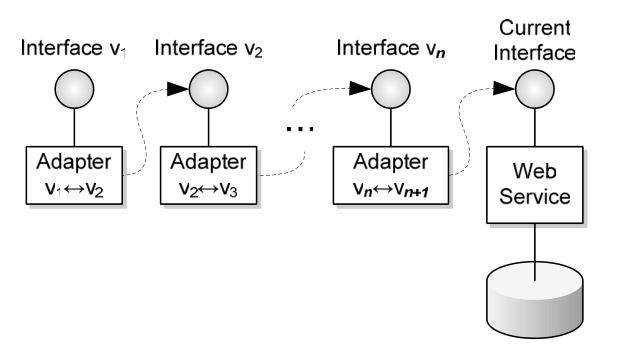
\includegraphics[height=2in]{chain}
    \caption{Chain of adapters structure
    after n versions have been published~\cite{13}}
    \label{fig:chain}
\end{figure}

Updating a service's API in this manner requires the developer to do two additional tasks:
\begin{itemize}
    \setlength\itemsep{0em}
    \item Duplicate all modified endpoints in service contract into a different path;
    \item Manually implement an adapter that translates the endpoints in version $v_i$\textrightarrow$v_{i+1}$.
\end{itemize}
The adapters code is included in the web service implementation that supports the revised service endpoints.
The adapters are not deployed separately, only the most up to date implementation of a service is deployed.

For instance, when an outdated consumer in version $v_i$ communicates with a producer in version $v_{i+2}$, the endpoints that provide the service
in version $v_i$ use the adapters $v_i$\textrightarrow$v_{i+1}$, and $v_{i+1}$\textrightarrow$v_{i+2}$ to translate the operation before forwarding it to the endpoint in the current version.

This approach offers a high degree of granularity because all types of contract evolutions can be supported under it.
The adapter's implementation are tailored to solve specific contract evolutions, allowing the developer to select the most appropriate evolution strategy and method.
However, it is difficult to maintain a system using this approach due to burden imposed by the additional tasks described above.

\subsection{Lazy Proxy Adapter} % (fold)
\label{sec:proxy_adapter}

In this strategy the knowledge of a microservice’s
contract is used to automatically create a lightweight proxy capable of dynamically adapting the messages exchanged between services to match them with the static service code.
The proxy intercepts messages from consumers and adapts the message to the new specification before they reach the producer.
Consumer services are initially deployed without the adapter proxy.
Proxies are installed and updated on demand using a lazy instantiation method, that builds and deploys the adapter proxy when the first communication between corresponding services occurs.
\citeauthor{seco2020robust} and \citeauthor{santosregent} investigate this approach \cite{seco2020robust, santosregent}.

The proxy creation mechanism makes use of the available meta-information
to automatically update the proxy components as needed.
In essence, every communication contains information about the agreed-upon version, the handshake protocol uses this information to determine if a proxy update is required or not.
The lazy instantiation method improves the maintainability of the system by
simplifying deployment operations.

This approach improves the system maintainability, by sacrificing some granularity on the supported evolutions due to the automatic generation of the proxy components.
However, with this approach external consumers cannot be served, since changes to a service contract affect its consumers.
The proxy adapter components cannot be easily installed in unsupervised consumers.

\section{Contract Evolution in MicroService Architectures} % (fold)
\label{sec:contract_evolution_in_microservice_architectures}

The evolution of a microservice contracts while ensuring their soundness and
avoiding heavy adaptation processes due to service redeploying is demonstrated to be possible by \citeauthor{seco2020robust} \cite{seco2020robust}.
The proposed approach to microservice contract evolution \cite{seco2020robust} makes use of a global deployment manager component that is responsible for managing module references,
as well, as dynamically generated proxies that are capable of adapting messages exchanged between modules when contracts mismatch.
The following example demonstrates the mechanism.

\begin{figure}[htbp]
    \centering
    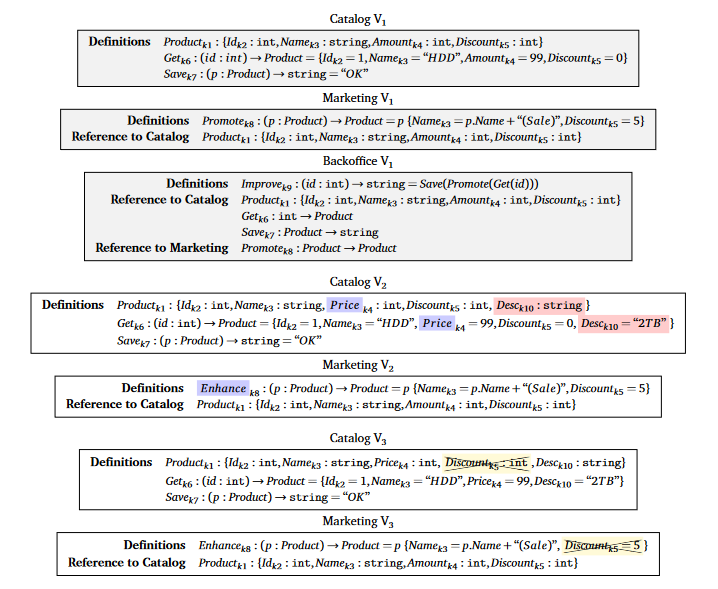
\includegraphics[height=5in]{adapter_example}
    \caption{Evolution of modules Catalog, Marketing, Backoffice \cite{seco2020robust}}
    \label{fig:evolution_of_modules}
\end{figure}

Consider the marketing system shown in Figure \ref{fig:evolution_of_modules} that comprises three distinct modules: Catalog, Marketing, and BackOffice.
These three simple modules combined, form a triangle of dependencies, complex enough to demonstrate the proposed mechanism.
Please note that the Catalog module is a producer, whereas the Marketing module is a producer and a consumer.

Each module has a unique name, a collection of type and function definitions, and a set of type and function references.
If a producer module exposes definitions, they can be used by other consumer modules via an explicit reference.
Each programming element is accompanied by an immutable and unique key; for instance – the key of type ''Product'' is k1.
These keys enable elements to be identified even after they have been renamed or reinstated.

Initially, the system is composed by a collection of services,
represented in grey in the first instance of the example.
The reference definitions indicate their interactions.

In a second phase, it is developed version 2 of the Catalog and Marketing modules independently.
In the Catalog module, the element ''Amount'' is renamed to ''Price'', and the attribute ''Desc'' is added, while in the Marketing module,
the attribute ''Promote'' is renamed to ''Enhance''.
The module BackOffice has not been modified at this point and will become out of sync with the other modules.
In the figure, the newly added and modified elements are highlighted in red and blue, respectively.

In a third phase, the Catalog module is upgraded to version 3, where the attribute ''Discount'' of the element ''Product'' is removed.
The elements that have been removed are highlighted in yellow.
This version cannot be deployed in conjunction with version 2 of Marketing, as the attribute is used by the function ''Enhance''.

Both modules can be deployed together if the attribute ''Discount'' is removed in the definition of ''Enhance'', resulting in version 3 of Marketing module.
Additionally, it can be deployed version 3 of Marketing first and then version 3 of Catalog, but not vice versa.
Furthermore, it is permitted to retain the attribute "Discount" in the specification of the type "Product" in the reference to catalog.
Correctness is guaranteed as long as the property is not utilized.

As illustrated,
the system is capable of overcoming differences in contract definitions with the following evolutions:
\begin{itemize}
    \item \textbf{Adding new attributes to a type -} As a result of the addition of the "Desc" attribute to Catalog, the data returned by this module will include values for this attribute.
    Other modules will keep this data (as unknown attributes) to ensure that no data is lost;
    \item \textbf{Renaming functions -} The ''Promote'' function in Marketing module has been renamed to ''Enhance'', which will affect the endpoints exposed by the service.
    The proxy is dynamically built at runtime to use the actual endpoint name while issuing calls, eliminating the need to update and redeploy the service Backoffice;
    \item \textbf{Eliminating unused attributes and functions -} Unused elements do not require explicit adaptation.
\end{itemize}

Traditional approaches, are insufficiently robust to handle these types of changes, effectively rendering them breaking changes.
For instance, renaming functions results in the modification of remote URIs, and changing the name of an attribute may result in data loss.
By contrast, with this approach, such changes are permitted without compromising module compatibility.
This adaptive approach enables gradual module deployment of the referenced modifications without halting the entire system, avoiding data loss and misinterpretations.

\section{Service Integration Adapters} % (fold)
\label{sec:service_integration_adapters}

There has been substantial investigation on the adaptability of services in the context of service-oriented architectures~\cite{adaptersWebServices}.
Although SOA and Microservices are similar in that they both use a separation approach based on services,
these two designs differ in several important ways, most notably in that microservices are loosely coupled whereas SOA services are tightly tied due to common data storage between services.
As a result, adaptability in SOA is focused on service integration and replace-ability rather than evolution.

In the setting of SOA, adapters are used to wrap the heterogeneous services that communicate with distinct protocols and data formats,
in order to make them homogeneous and integrated them more easily.
These adapters presume that data adaptation has already been established by developers at an upper layer,
their primary concern is integrating services with distinct communication protocols and mismatches between operations that have the
same functionality but different signatures (e.g\ parameters name, order, type).

\citeauthor{adaptersWebServices}~\cite{adaptersWebServices} present a taxonomy of all conceivable mismatches as well as remedies to each type in the context of SOA.
Some of the defined mismatches remain important in the context of microservice evolution:
\begin{itemize}
    \item \textbf{Message Split Mismatch:} This type occurs when the protocol P requires a single message to achieve certain functionality,
    while in protocol PR the same behavior is achieved by receiving several messages.
    \item \textbf{Message Merge Mismatch:} This type occurs when protocol P needs to receive several messages for achieving certain
    functionality while protocol PR requires one message to achieve the same functionality.
    \item \textbf{Differences at the Operation Level:} This type occurs when the operation O of service S imposes constraints on input parameters,
    which are less restrictive than those of operation O input parameters in service SR (e.g., differences in value ranges).
\end{itemize}

The ''Message Split Mismatch'' can be handled through an adapter, however doing so
would require the adapter to use distributed transactions in order to handle independent failures in each contacted service.

The ''Message Merge Mismatch'' can also be solved with an adapter, but the adapter must be stateful because it must store request messages before they can be merged and sent through the new endpoint.

The first two types of mismatches can be handled in the context of microservice evolution without the aforementioned complications,
by essentially keeping the old endpoints operational but marked as deprecated until  there are no more consumers using them, and by providing the new endpoints in parallel.

The latter form of mismatch ''Differences at the Operation Level'' has an impact on microservice evolution if service contracts allow refined types.
In other words, when constraints in input parameter are validated in a layer above the application layer.
If validation is conducted in a lower layer, the mismatch can be easily resolved by modifying the application's implementation while keeping the service contract untouched.

\section{Deployment Strategies} % (fold)
\label{sec:deployment_strategies}

Deployment strategies~\cite{deploymentstrategies} are techniques that aim to provide means to upgrade a service,
while discontinuing the previous implementation without incurring downtime.

These strategies will be beneficial in the context of the proposed solution since all service updates will evolve the immediate termination of the prior implementation,
as it is no longer required to keep several versions available to offer backwards compatibility in service contracts.

A blue-green deployment approach is the most often used deployment strategy.
The new version ''blue'' is made available for testing and review, while users continue to use the stable version ''green''.
Users are migrated to the new version after it has passed all compliance tests.

A common alternative strategy is to have two A/B versions active at the same time, with some users using one and others using the other.
This strategy can be used to test and gather feedback on modifications to user interfaces.
It can also be used to troubleshoot problems that affect only a subset of users, in a production setting.

A canary deployment can be used to evaluate a new version, if a problem is discovered, the deployment is quickly reverted.
This technique can be performed in either of the above approaches.

A rolling deployment is an alternative strategy that gradually replaces instances of a service previous version with instances of the new version.
Before scaling down the old components, a rolling deployment normally waits for additional pods to become available through a readiness check.
If a significant problem arises, the rolling deployment is halted.
This strategy ensures the highest availability while using the fewest resources.
In comparison to other strategies, the additional resources allocated during the deployment process are minimal.

\section{API Management Tools} % (fold)
\label{sec:api_management_tools}

API management is the process of overseeing functions like API creation, description, testing, analysis, publication, securing, and monitoring.
All of these functions can only be met with the assistance of tools.

Microsoft Azure's API Management Platform (AAMP)~\cite{azureapi} is an example of a system that provides tool's with the functionalities mentioned above.
For example, in this platform, programmers are allowed to specify transformations in policy statements, that are performed on all responses from a microservice.
The main use case of these transformations in AAMP is the integration of legacy backends by modernizing their APIs and making them accessible from cloud services, without the risk of migration.
This tool is one of the inspirations for the proposed approach, which aims to allow similar transformations to be
performed in both request and response messages.

In AAMP all requests from client applications are routed through the API gateway, which then forwards them to the appropriate backend services.
The API gateway, acts as a facade to the backend services,
allowing API providers to abstract API implementations and evolve backend architecture without impacting API consumers.
The AAMP's other responsibilities and functionalities include:
\begin{itemize}
    \setlength\itemsep{0em}
    \item Accepting API calls and routing them to configured backends;
    \item Verifying API keys, JWT tokens, certificates, and other credentials;
    \item Enforcing usage quotas and rate limits;
    \item Caching responses to improve response latency and minimize the load on backend services;
    \item Emitting traces for monitoring, reporting, and troubleshooting;
    \item Collecting API usage metrics.
\end{itemize}

Most of the aforementioned functionalities are also supported in the Kubernetes ecosystem and its extensions.
The proposed approach can be viewed as API management tool that solely focus on the evolution of API's.
We aim to make it compatible with existing API management tools in the Kubernetes ecosystem that cover the other functionalities.
